%! TEX root = ../../main.tex

\subsection{Kubernetes}%
\label{sub:Kubernetes}

The practise of running microservices in a production environment is not only
used by big technology companies. The United Kingdom government's Department
for Work and Pensions states to be running one of the largest microservice
architectures in Europe. The country's public services \textit{universal
credit} system fully runs as a microservice architecture
\autocite{LoweLeadingwaymicroservices2016}. Yet how is it possible to
orchestrate such a huge amount of microservices?

Kubernetes is a container orchestration solution that is capable of
automatically deploying, scaling and managing containers
\autocite{AuthorsProductionGradeContainer}. It was introduced in 2014 by Google
and is based on the experience Google gained while developing among other
things \textit{Borg} and \textit{Omega}. Borg and Omega were applications
internally developed by Google to manage their thousands of applications and
services \autocite{LuksaKubernetesAction2017}.

This chapter will shortly introduce the main concepts of Kubernetes and give an
overview of the Kubernetes components that are relevant to the research
questions. If needed, The official Kubernetes documentation
\autocite{AuthorsProductionGradeContainer}, which covers all system components
in detail, can be used as a supplement to this thesis.

\subsubsection{Concepts}%
\label{ssub:Concepts}
Kubernetes distinguishes between \textit{master} and \textit{node} components.
The master components, also referred to as \textit{control plane}, are in
charge of managing a cluster. The control plane hosts Kubernetes' API, manages
the clusters configuration and schedules \textit{pods} to run on available
nodes \autocite{AuthorsKubernetesComponents2019}. In general, the master
components are responsible for keeping the cluster alive.

The node components on the other hand are executed on every node of the
cluster. Any node of a Kubernetes cluster runs an agent, \textit{kubelet}, that
ensures that all containers of the node's assigned pods are executed. Further,
a node always runs the network proxy \textit{kube-proxy} that enforces
networking rules and manages the node's traffic. Lastly, a container runtime
allows all of this to happen. As already mentioned in
Chapter~\ref{ssub:Deployment_Runtime_Model}, there are several runtime
environments to chose from. Next to Docker, Kubernetes also directly supports
\textit{containerd}, \textit{crio-o}, \textit{rktlet}
\autocite{AuthorsKubernetesComponents2019}.

\paragraph{Pods}%
\label{par:Pods}
Instead of directly deploying individual containers, Kubernetes introduces the
concept of \textit{pods}. A pod is the smallest entity that can be executed on
the cluster. It hosts at least one containers and automatically receives a
\ac{IP} address that is unique inside Kubernetes. Kubernetes ensures that all
containers of a pod are always executed in the same node.

Yet this does not mean that a complete microservice architecture should be
bundled into one pod. The decision when to combines microservices into one pod
and when to split them across multiple pods becomes clear in the following
example. Given is an exemplary microservice architecture consisting of a basic
web crawler that fetches all \textit{xkcd} comics from the xkcd archive and
stores them in the file system, a frontend that displays the fetched comics and
a backend that serves the fetches images to the frontend. The architecture is
also depicted in figure~\ref{fig:pods_example}. Both the backend as well as the
crawler have to access the same file system. Further, the backend would not be
able to serve comics without the crawler hence it would fail to fulfil its
task. Thus it can be said that these two services are \textit{tightly coupled}
and are a dependent components. It can also be argued that the crawler only
acts as a supporting component for the actual backend. Hence, the crawler and
backend should be shipped inside the same pod. On the other hand the frontend
is a fully independent system component. It can be scaled independently from
the backend and crawler. Hence it belongs in a separate pod. 

\begin{figure}[H]
\begin{center}
  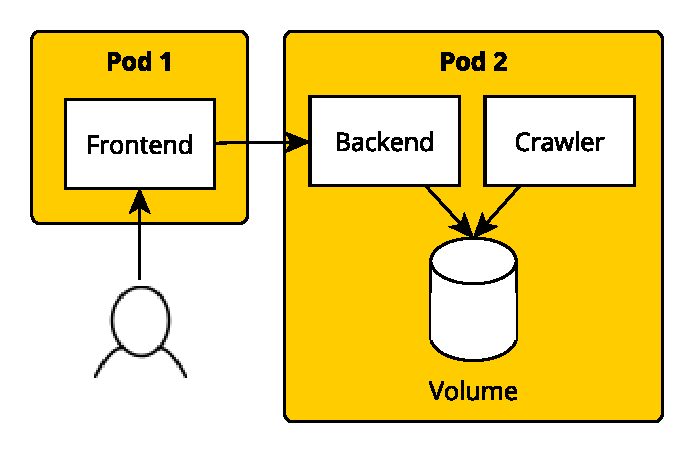
\includegraphics[scale=0.7]{images/figures/pod_example.pdf}
\end{center}
\caption{Example microservice architecture displayed as pods, containers and a volume.}%
\label{fig:pods_example}
\end{figure}

\paragraph{Volumes}%
\label{par:Volumes}

The example in figure~\ref{fig:pods_example} also introduces the concept of
\textit{volumes}. Volumes bring the ability to store files \textit{outside} the
context of the local file system of a container. A pod can specify that it
needs one or more volumes. Each container inside a pod is able to mount these
volumes in the same or a different. The backend from
figure~\ref{fig:pods_example} might mount the volume to
\texttt{/var/www/storage} whereas the crawler wants to mount the volume to
\texttt{/mnt/comics}. Volumes are either local paths on the Kubernetes node or
are maintained by a cloud provider's service like e.g. \textit{Microsoft Azure
File Volumes}.

Simply using the Kubernetes concept of volumes however does pose two significant problems:
\begin{itemize}
  \item For most volume types, the volume has to be provisioned by hand before
    the container can allocate said volume.
  \item The volume is bound to the pods lifecycle. This means that whenever a
    pod is deleted or e.g.\ dies due to a problem or scaling, the volume needs
    to be recreated during the pod's next startup. This also means that volumes
    can not be defined without first defining a pod.
\end{itemize}

\paragraph{Persistent Volumes, Persistent Volume Claims and Storage Classes}%
\label{par:Persistent_Volume_Claims_and_Storage_Classes}
One way to solve these problems is to use \textit{\acfp{PV}}. A \ac{PV} can be
defined without first having to define a pod. While it is possible to
statically define a set of \acp{PV}, it is useful to let Kubernetes dynamically
provision \acp{PV} when needed.

\begin{figure}[H]
\begin{center}
  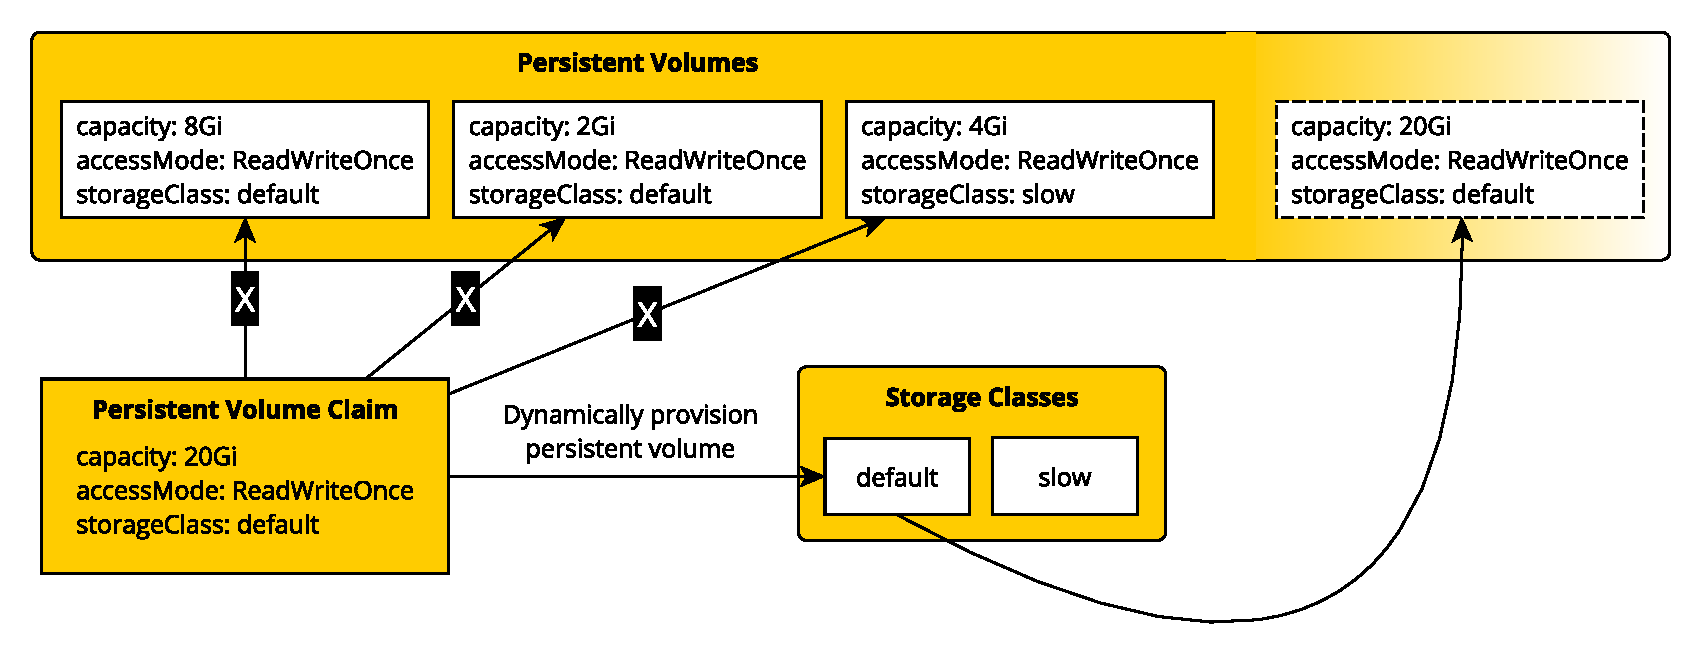
\includegraphics[scale=0.5]{images/figures/pvs.pdf}
\end{center}
\caption{The process of dynamically provisioning a \acf{PV} using a \acf{PVC}.}%
\label{fig:dynamic_pvs}
\end{figure}

Figure~\ref{fig:dynamic_pvs} shows the process of how Kubernetes dynamically
provisions \acp{PV}. To understand this flow of actions, two terms have to be
defined: \textit{\acf{PVC}} and \textit{storage classes}. 

A \ac{PVC} is a request for an available \ac{PV}. It can specify, among other
things, an access mode and resources. Contrary to pods which can request
computing resources, \acp{PVC} request storage resources. Additionally, the
\ac{PVC} can request a specific storage class and a selector that must match
the \ac{PV}'s label. Only if the selector matches the \ac{PV}'s label, the
\ac{PV} is capable of resolving the \ac{PVC}.

A storage class abstracts the different options of storage available in a
cluster. Any storage class is supported by a \textit{provisioner} that is
responsible for handling the actual storage; e.g.\ CephFS handles storage
differently from GlusterFS. Thus storage classes are the underlying foundation
for all persistent volumes inside Kubernetes. A crucial property of storage
classes are their \textit{reclaim policy}. The reclaim policy determines
whether a \ac{PV} deployed on a storage class is \textit{deleted} or
\textit{retained} once the \ac{PV}'s \ac{PVC} is released. Thus the reclaim
policy ultimately defines the persistency of a \ac{PV} beyond the lifecycle of
a \ac{PVC}. Additionally whenever a new \ac{PVC} is created that matches the
originally described selector and storage class, a retained \ac{PV} can be
reallocated by the \ac{PVC}.

The behaviour in figure~\ref{fig:dynamic_pvs} should now become clear.
Kubernetes tries to assign an available, non-bound \ac{PV} to the \ac{PVC}.
The existing ones however do not match the requirements set by the \ac{PVC}. To
solve this, a new \ac{PV} is automatically provisioned that fully complies with
the requirements of the \ac{PVC}.

To conclude this section, it can be said that \acp{PV} bring the ability of
storage resource definition that is independent from a pod's lifecycle.
\acp{PVC} can then be used to allocate the created \acp{PV} or dynamically
create new ones by using the storage classes' provisioner.

\paragraph{Controllers: StatefulSets, ReplicaSets and Deployments}%
\label{par:Controllers}
Pods, as they were introduced in the~\ref{par:Pods} section of this chapter,
are fully unmanaged. The downside to this is that whenever a node dies, all
pods running on this node also die without getting redeployed on a healthy
node. Additionally, unmanaged pods can not be be scaled automatically by
Kubernetes. It is also not possible to schedule unmanaged pods to run
periodically \autocite[Ch. 4]{LuksaKubernetesAction2017}. Kubernetes solves
these issues by introducing a new concept: controllers. Controllers are
responsible for managing a set of Kubernetes resources and extend their
original capabilities \autocite{AuthorsConcepts2019}. This sectional will
briefly cover the controllers needed for this thesis. Next to the highlighted
controllers, Kubernetes includes a number of other controllers that are listed
in \autocite{AuthorsConcepts2019}.

Instead of scaling pods manually to ensure the accessibility to a service, a
ReplicaSet manages a set of pods and ensures that a specified number of
replicas of these pods is always available. The discovery of pods that should
be managed by a ReplicaSet is based on \textit{selectors}. If a ReplicaSet's
selector matches the label of a pod and the pod is not already assigned to a
different controller, the ReplicaSet takes ownership of said pod \autocite[Ch.
4]{LuksaKubernetesAction2017}. Hence any pod that may not be managed by a
ReplicaSet has to define another label in order not to be make subject to a
ReplicaSet~\ref{AuthorsReplicaSet2019}. Additionally to owning pods that only
match the ReplicaSet's selector, it is possible to directly specify pods that
should be spawned whenever the ReplicaSet is loaded. This option is more common
and directly highlights the pod's connection to the ReplicaSet
\autocite{AuthorsReplicaSet2019}. In addition, \autocite{AuthorsReplicaSet2019}
discourages from directly using ReplicaSets if the use case does not need a
custom update logic. Instead, it is recommended to use \textit{deployments}.

A deployment is a higher-level abstractional concept that itself manages
ReplicaSets \autocite{AuthorsReplicaSet2019}. Contrary to the ReplicaSet, a
deployment is able to update all its managed pods and roll back changes to a
previous state. All changes can be performed declaratively without having to
write any logic; this process is managed by Kubernetes \autocite[Ch.
9]{LuksaKubernetesAction2017}.

 % Add more information about the rolling update process.

Both the ReplicaSet and deployment are meant to be used for stateless
applications. Each pod that is managed by either one of these controllers does
not have an individual identity. Hence, it is not possible to identify a single
managed pod; they all look and behave exactly the same. All pods also share the
same persistent volume. The question arising from this is how a distributed
application that needs stateful and distinct entities, i.e.\ a database system
using the master/slave paradigm, can be hosted using Kubernetes. In the
master/slave paradigm, the master nodes are responsible for managing the
databases data. The slaves then replicate the data and can be used for i.e.\
reliably reading data and balancing the reading load. Yet, this scenario brings
up three problems that can not be easily solved with a ReplicaSet or
deployment. The problems are named $P_x$ for future reference.

\begin{itemize}
  \item \textbf{$P_1$}: Each pod needs its own storage volume to avoid lock problems.
  \item \textbf{$P_2$}: Each pod needs to be addressed individually so that the master(s) are
    capable of syncing data to only selected slave(s).
  \item \textbf{$P_3$}: After a pod dies, Kubernetes has to spawn a pod with
    the same identity. This is the only way to guarantee that the master(s)
    get respawned with the same data and that slave(s) do not have to rejoin
    the database cluster and resync all data.
\end{itemize}

Even though \autocite[Ch. 10]{LuksaKubernetesAction2017} lays out options to
solve these problems using ReplicaSets, a new component is needed to solve them
sustainably - entering StatefulSets. 

\begin{figure}[H]
  \begin{center}
  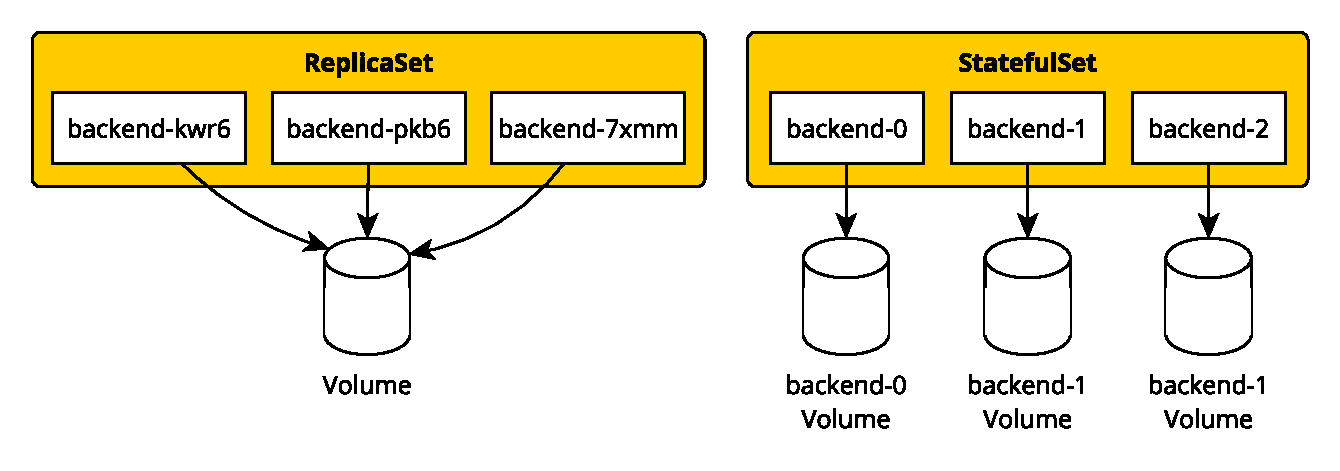
\includegraphics[scale=0.7]{images/figures/statefulSets_vs_replicaSets.pdf}
\end{center}
\caption{A comparison of ReplicaSets and StatefulSets.}%
\label{fig:statefulSetsVSReplicaSets}
\end{figure}

In a StatefulSet, each managed pod receives its own identity. Instead of
randomly assigning names and \ac{IP} addresses to pods, their names are
numbered. A custom identity also means a seperate volume from the rest of the
pods inside the StatefulSet. Whenever the StatefulSet needs to redeploy a pod
(e.g.\ due to a node that went down or due to scaling) the respawned pods
receive the same identity they had before. In
figure~\ref{fig:statefulSetsVSReplicaSets} this would mean that if
\texttt{backend-2} went offline due to a faulty host, the StatefulSet would
spawn an exact copy of \texttt{backend-2} with the same identity (meaning name,
\ac{IP} and volume). Hence, it can be argued that StatefulSets solve problems
$P_1$-$P_3$ that could not be easily solved by ReplicaSets. They are the way to
go when deploying stateful applications that may require unique pod identies.

\paragraph{Services}%
\label{par:Services}
Regardless of the controller managing the replication of pods, a solution is
needed to address any given set of pods. When e.g.\ scaling a set pods of
ReplicaSet to 15 instances how should a user sent a request to either one of
them without addressing each one individually. Services expose a set of pods to
the network as an \ac{IP} address and name that can be resolved inside the
cluster.
